Consider a dataset consisting of points in the form of $(x, y)$, where $x$ is a real value, and $y \in \{-1,\ 1\}$ is the class label. There are only three points $(x_1, y_1) = (-1,\ -1),\  (x_2, y_2) = (1, -1)$, and $(x_3, y_3) = (0,\ 1)$, shown in Figure~\ref{line_plot1}.

\vspace{0.3cm}
\begin{figure}[htbp] 
	\centering
	
\includegraphics[width = .6\textwidth]{svm_line.png}
	\caption{Three data points considered in Problem 1}
	\label{line_plot1}
\end{figure}

\textbf{1.1} (\blue{2pts}) Can these three points in their current one-dimensional feature space be perfectly separated with a linear classifier? Why or why not?\\

\noindent{\fontsize{11}{12}\selectfont\textbf{Solution 1.1}}

Answer: No, it cannot. This is so because these three points are not linearly separable in a 1D space.
\bigskip
Proof by Contradiction:
Suppose that these three points are linearly separable. Then exist a liner separator that:
\[
f(x)=sign(wx+b)
\]
which means:
\[
y_i(wx_i+b)> 0 \textbf{ \; for all i}
\]
Then we have:
for point (-1, -1)
\begin{align*}
-1(w(-1)+b)>0 \\
\rightarrow w>b
\end{align*}
for point (1, -1)
\begin{align*}
-1(w(1)+b)>0 \\
\rightarrow w+b<0
\end{align*}
for point (0, 1)
\begin{align*}
1(w(0)+b)>0 \\
\rightarrow b>0
\end{align*}
sum up:
\begin{align*}
&(1) \; w>b \\
&(2) \;w+b<0 \\
&(3) \;b>0 \\
\end{align*}
conjugate (1) and (3) we have:
\[
w>b>0 \rightarrow   w>0 \;(4)
\]
(3) and (4) conjugate leads to a contradiction to (2):
\begin{align*}
&(4) \; w>0 \\
&(3) \;b>0 \\
&\rightarrow w+b > 0 
\textbf{\; \; and also \; }w+b<0 \;(4)
\end{align*}

Since any threshold will leave at least one negative point on the same side as the positive point, thus, perfect linear separation is impossible.

\bigskip

\textbf{1.2} (\blue{3pts}) Now we define a simple feature mapping $\mathbf{\phi}(x) = [x, x^2]^T$ to transform the three points from one-dimensional to two-dimensional feature space. Plot the transformed points in the new two-dimensional feature space. Is there a linear model $\w^T\x +b$ for some $\w\in \R^2$ and $b \in \R$ that can correctly separate the three points in this new feature space? Why or why not?\\

\noindent{\fontsize{11}{12}\selectfont\textbf{Solution 1.2}}
first, mapping: $\mathbf{\phi}(x) = [x, x^2]^T$
\begin{align*}
&\mathbf{\phi}(-1, -1) \rightarrow  (-1,1) \textbf{\; label: $-1$}\\
&\mathbf{\phi}(1, -1) \rightarrow (1,1) \textbf{\; label: $-1$}\\
&\mathbf{\phi}(0, 1) \rightarrow (0,0) \textbf{\; label: $1$}
\end{align*}

\begin{figure}[htbp]
\centering
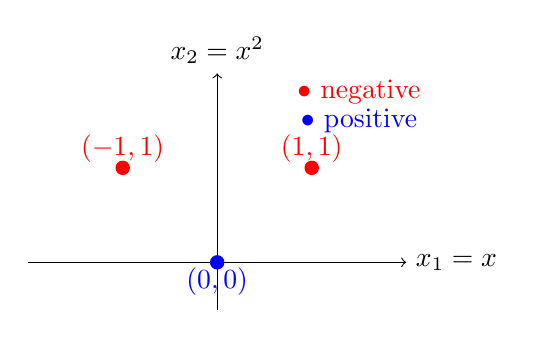
\begin{tikzpicture}[scale=1.2]

% Axes
\draw[->] (-2,0) -- (2,0) node[right] {$x_1 = x$};
\draw[->] (0,-0.5) -- (0,2) node[above] {$x_2 = x^2$};

% Negative class points (-1)
\filldraw[red] (-1,1) circle (2pt);
\filldraw[red] (1,1) circle (2pt);

% Positive class point (+1)
\filldraw[blue] (0,0) circle (2pt);

% Labels
\node[red] at (-1,1.2) {$(-1,1)$};
\node[red] at (1,1.2) {$(1,1)$};
\node[blue] at (0,-0.2) {$(0,0)$};

% Legend
\node[red] at (1.5,1.8) {$\bullet$ negative};
\node[blue] at (1.5,1.5) {$\bullet$ positive};

\end{tikzpicture}
\caption{Transformed points in the 2D feature space $\phi(x) = (x,x^2)$.}
\end{figure}

Obviously there are margins between negative and positive points. Thus, there are multiple linear model can correctly separate points.

For example (also the max margin): $y= 0.5$
Let $w=(0,1)^T$ and $b= -0.5$

For these three points:
\begin{align*}
&(-1,1) :  \; 0+ 1-0.5=0.5>0 \\
&(1,1) :  \;  0+ 1-0.5=0.5>0 \\
&(0,0) :  \;  0- 0.5= -0.5<0
\end{align*}
This will enable the classification symbols to match the labels. 
The mapping $\mathbf{\phi}(x) = [x, x^2]^T$ lifts the data into a higher-dimensional space where the positive point lies below the two negative points. A linear boundary in this 2D space can easily separate them. A linear classifier, such as a horizontal line separating the origin from the points at $y=1$, can perfectly separate the classes. Therefore, the data become linearly separable after the feature transformation.

\bigskip

\textbf{1.3} (\blue{2pts}) Given the feature mapping $\mathbf{\phi}(x) = [x, x^2]^T$, write down the $3 \times 3$ kernel/Gram matrix $\mathbf{K}$ for this
dataset.\\

\noindent{\fontsize{11}{12}\selectfont\textbf{Solution 1.3}}
Write the kernel with the formular:
\[
K_{ij} = \phi(x_i)^\top \phi(x_j)
\]
\[
K_{ij}
=
\phi(x_i)^\top \phi(x_j)
=
x_i x_j + x_i^2 x_j^2.
\]
for $x_i = {-1, 0, 1}$
\begin{align*}
K_{ij} =& x_i x_j + x_i^2 x_j^2 \\
=& (-1)(-1) + 1*1= 2 , (-1) (0) + 0= 0, (-1)(1)+ (1)(1) = 0,\\
   & ......  \\
\textbf{Therefore:}\\
K_{ij} = 
&\begin{pmatrix}
2 & 0 & 0 \\
0 & 0 & 0 \\
0 & 0 & 2 \\
\end{pmatrix}
\quad \textbf{or as previous x $\in$ (-1,1,0) }
\quad \begin{pmatrix}
2 & 0 & 0 \\
0 & 2 & 0 \\
0 & 0 & 0 \\
\end{pmatrix}
\end{align*}

\bigskip

\textbf{1.4} (\blue{4pts}) Now write down the primal and dual formulations of SVM for this dataset
in the two-dimensional feature space.
Note that when the data is separable, we set the hyperparameter $C$ to be $+\infty$
which makes sure that all slack variables ($\xi$) in the primal formulation have to be $0$
(and thus can be removed from the optimization).\\

\noindent{\fontsize{11}{12}\selectfont\textbf{Solution 1.4}}

Since the data points can be separable under $\mathbf{\phi}(x)$, the primal formulations of SVM is optm ($\xi =0$).
\[
\begin{aligned}
\min_{w,b} \quad & \frac{1}{2}\|w\|^2 \\
\text{s.t.} \quad 
& y_i \big(w^T \phi(x_i) + b\big) \ge 1, 
\quad i = 1,2,3
\end{aligned}
\]
For these three points:
\begin{align*}
(-1,1) :  &\; -1(w_1(-1)+w_2(1)+b) \ge 1 \\
(1,1) :  &\;  -1(w_1(1)+w_2(1)+b) \ge 1 \\
(0,0) :  &\;  1(w_1(0)+w_2(0)+b) \ge 1
\end{align*}

And dual formulations of SVM.
\[
w^{(t)} = \sum_{i=1}^{n} a_i^{t} y_i \phi(x_i)
\]
\begin{center}
to
\end{center}
\[
\begin{aligned}
\max_{\alpha} \quad 
& \sum_{i=1}^{3} \alpha_i
- \frac{1}{2}
\sum_{i,j=1}^{3}
\alpha_i \alpha_j y_i y_j K_{ij} \\
\text{subject to} \quad
& \sum_{i=1}^{3} \alpha_i y_i = 0,
\quad \alpha_i \ge 0.
\end{aligned}
\]
Since we have $K_{ij}$ from 1.3, bring in three points:
\[
\begin{aligned}
\max_{\alpha_1,\alpha_2,\alpha_3}
\quad
&\alpha_1 + \alpha_2 + \alpha_3
-
\frac{1}{2}
\left( 2\alpha_1^2 + 2\alpha_2^2 \right) \\
\text{subject to} \quad
& \alpha_3 = \alpha_1 + \alpha_2,
\quad \alpha_i \ge 0.
\end{aligned}
\]


\bigskip

\textbf{1.5} (\blue{5pts}) Next, solve the dual formulation exactly (note: while this is not generally feasible, the simple form of this dataset makes it possible).
Based on that, calculate the primal solution.\\

\noindent{\fontsize{11}{12}\selectfont\textbf{Solution 1.5}}

From 1.4 we easily to have:
\[
\begin{aligned}
\max_{\alpha_1,\alpha_2,\alpha_3}
\quad
&\alpha_1 + \alpha_2 + \alpha_3
-
\frac{1}{2}
\left( 2\alpha_1^2 + 2\alpha_2^2 \right) \\
\text{subject to} \quad
& \alpha_3 = \alpha_1 + \alpha_2,
\quad \alpha_i \ge 0.
\end{aligned}
\]

Thus,
\[
\begin{aligned}
\max_{\alpha_1,\alpha_2,\alpha_3}
\quad
&\alpha_1 + \alpha_2 + \alpha_1 + \alpha_2 -\alpha_1^2 + \alpha_2^2  \\
\text{subject to} \quad
&\quad \alpha_i \ge 0.
\end{aligned}
\]
Leads to
\[
\begin{aligned}
\hat{g}(\alpha_1 , \alpha_2) = \;
&(2\alpha_1-\alpha_1^2) + (2\alpha_2 - \alpha_2^2)  \\
\text{subject to} \quad
&\quad \alpha_i \ge 0.
\end{aligned}
\]
Find the derivative of $a_i$ equals to 0 for $\hat{g}$:
\[
\begin{aligned}
&\frac{d}{d_{ai}} \hat{g} =  \frac{d}{d_{ai}}(2a_i - a_i^2) = 2-2a_i +0 = 0;  \quad \longrightarrow \quad
a_i =1  \quad (i = 1, 2). \\
&\textbf{bring back to constrain} \\
&a_3 = a_1 + a_2 = 2
\end{aligned}
\]
Which all $a_i$ satisfies the non-negative constraint. Thus, the optimal solution is,
\[
a_1 = 1, a_2 = 1, a_3 = 2
\]

\textbf{Then restore the primal solution from the dual solution:}
\begin{align*}
w^{*} &= \sum_{i=1}^{3}  a_i^{*} y_i \phi(x_i) \\
&= 1(-1)[-1,1]^T + 1(-1)[1,1]^T + 2 (1) [0,0]^T = [1,-1]^T + [-1,-1]^T + [0,0]^T \\
&=  [-1+1+0,-1-1+0]^T = [0,-2]^T
\end{align*}
Calculate the bias $b^{*}$ based on the constraint of the support vectors:
\[
y_i \big(w^{*T} \phi(x_i) + b^{*}\big) = 1, 
\quad i = 1,2,3
\]
For $i = 1,2$ (should be same):
\begin{align*}
& -1 \big([0,-2]^T [-1,1] + b^{*}\big) = 1 \\
& 2 - b^{*} = 1 \quad \rightarrow \quad b^{*} = 1  \\
& -1 \big([0,-2]^T [1,1] + b^{*}\big) = 1 \\
& 2 - b^{*} = 1 \quad \rightarrow \quad b^{*} = 1  \\
\end{align*}
The final primal solution is
\[
w^{*} = [0,-2]^T ,  b^{*} = 1 
\]
Thus, $\|w^{*}\| = 2$ , the margin is $\frac{1}{\|w^{*}\|} = \frac{1}{2}$

\bigskip

\textbf{1.6} (\blue{3pts}) Plot the decision boundary (which is a line) of the linear model ${\w^*}^T \x + b^*$ in the two-dimensional feature space, where $\w^*$ and $b^*$ are the primal solution you got from the previous question. Then circle all support vectors. Finally, plot the corresponding decision boundary in the original one-dimensional space (recall that the decision boundary is just the set of all points $x$ such that ${\w^*}^T \mathbf{\phi}(x) + b^* = 0$).\\

\noindent{\fontsize{11}{12}\selectfont\textbf{Solution 1.6}}

The decision function in the original input space is
\[
f(x) = \mathbf w^{*\top}\phi(x) + b^*.
\]
Since
\[
\mathbf w^* = \begin{bmatrix}0\\-2\end{bmatrix},
\quad
\phi(x)=\begin{bmatrix}x\\x^2\end{bmatrix},
\quad
b^* = 1,
\]
we obtain
\[
f(x) = 0\cdot x -2x^2 + 1 = 1 - 2x^2.
\]

The decision boundary satisfies
\[
f(x)=0,
\]
which gives
\[
1 - 2x^2 = 0
\quad\Rightarrow\quad
x^2 = \frac12
\quad\Rightarrow\quad
x = \pm \frac{1}{\sqrt{2}}.
\]

\noindent{\textbf{Solution 1.6 (plot)}}

\begin{figure}[ht]
  \centering
  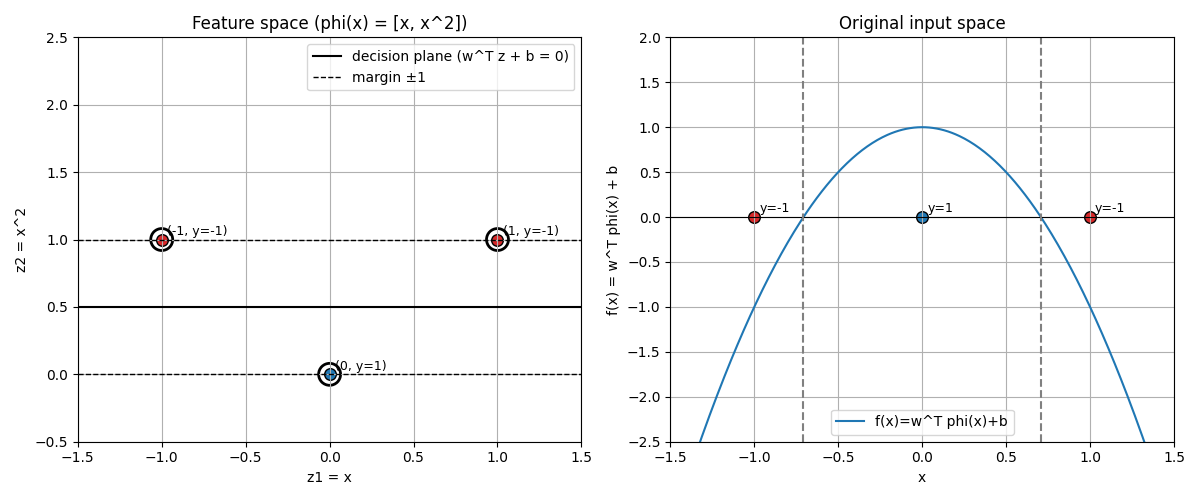
\includegraphics[width=0.9\textwidth]{Figure_1.png}
  \caption{Left: feature space $z=\phi(x)=[x,x^2]^\top$ showing the linear decision plane $w^{*\top}z+b^*=0$ (solid), margins $=\pm1$ (dashed), and support vectors (circled). Right: original input space showing $f(x)=w^{*\top}\phi(x)+b^*=1-2x^2$ and the decision boundary $x=\pm 1/\sqrt{2}$.}
  \label{fig:svm_plots}
\end{figure}


\bigskip
